%! Author = timbe
%! Date = 05.02.2024

% Preamble
\documentclass[12pt]{article}

% Packages
\usepackage[left=3.0cm, right=1.5cm, top=2.0cm, bottom=2.0cm]{geometry}

\usepackage[utf8]{inputenc}
\usepackage[T2A]{fontenc}
\usepackage[russian]{babel}
\usepackage{amsmath, amsfonts, amssymb}
\usepackage{graphicx}
\usepackage{wrapfig}
\usepackage{fancyhdr}
\usepackage[shortlabels]{enumitem}
\usepackage{svg}
\usepackage{amstex}
\usepackage{colortbl}
\usepackage{bm}

\renewcommand{\vec}{\textbf}
\newcommand{\cross}{\times}

\pagestyle{fancy}
\fancyhead[L]{Работа №4.2.3}
\fancyhead[R]{Белинский Т.Д.\quad Б05-206}

% Document
\begin{document}
    \section*{4.2.3. ИНТЕРФЕРОМЕТР РЕЛЕЯ}
    \ \par
    \textbf{Цель работы:} ознакомление с интерференцией на двух щелях,
    устройством и принципом действия интерферометра Релея и с его
    применением для измерения показателей преломления газов. \par
    \textbf{Оборудование:} технический интерферометр ИТР-1, светофильтр,
    баллон с углекислым газом, сильфон, манометр, краны.

    \subsection*{Теоретическая часть}
    \ \par
    \textbf{Зависимость показателя преломления газа от давления и температуры.}
    Воспользуемся известной формулой диэлектрической проницаемости $\varepsilon$ для газа невзаимодействующих диполей:
    \[\varepsilon = n^2 = 1 + 4 \pi N \alpha,\]
    где $N$-- концентрация молекул, $\alpha$ -- поляризуемость молекулы (в ед. СГС).
    Эта формула справедлива для разреженных газов, и коэффициент преломления их мало отличается от единицы.
    Учитывая зависимость давления $P$ газа от температуры $P = N k_{\text{Б}}T$ , где $k_\text{Б}$ --
    константа Больцмана, получим соотношение
    \[n - 1 \approx \frac{\alpha}{2 k_{\text{Б}}T}P.\]
    Тогда для разности показателей преломления $\delta n = n_2 - n_1$, измеряемой с помощью интерферометра Релея,
    и разности давлений $\delta P$, измеряемой с помощью манометра, имеем простое соотношение:
    \[\delta n = \frac{\alpha}{2 k_{\text{Б}}T} \delta P\]


    \subsection*{Экспериментальная установка}
    \ \par
    Интерферометр Релея — прибор для измерения разности показателей преломления —
    основан на явлении дифракции света на двух параллельных щелях.
    Схема прибора представлена на рис.\ \ref{fig:fig1} в вертикальной и горизонтальной проекциях.
    Лампа накаливания $\text{Л}$ с помощью конденсора $K$ ярко освещает узкую входную щель $S$,
    расположенную в фокусе объектива $O_1$ (фокусное расстояние $f$).
    Коллиматор, состоящий из щели $S$ и объектива $O_1$, посылает параллельный пучок
    на диафрагму $D$ с двумя вертикальными щелями (расстояние между щелями $d$).
    Свет после двойной щели проходит кювету $L$, состоящую из двух одинаковых стеклянных камер,
    в которые вводятся исследуемые газы (в нашей установке — $CO_2$ или воздух).
    Кювета занимает только верхнюю часть пространства между объективами $O_1$ и $O_2$, длина кюветы $l$.
    За кюветой расположены две стеклянные пластинки $J$ (компенсатор Жамена, см. ниже) и пластинка $\text{П}$.

    \begin{figure}[h]
        \centering
        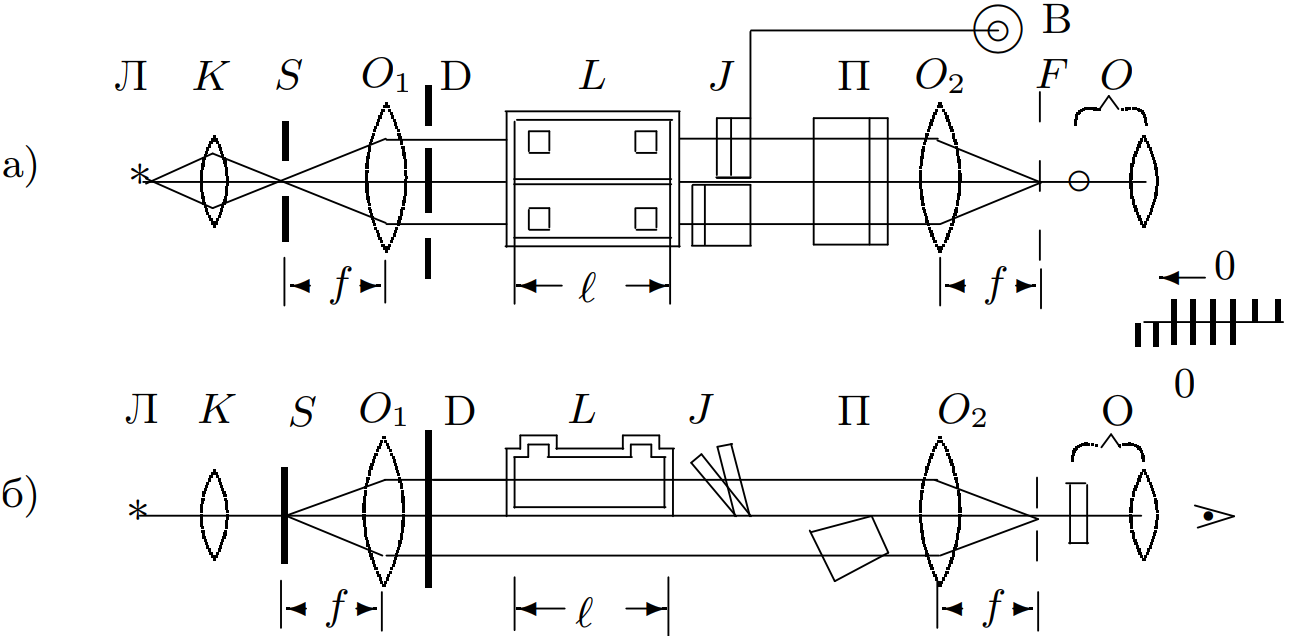
\includegraphics[width=0.8\linewidth]{pic/setup}
        \caption{Устройство интерферометра Релея: a) вид сверху; б) вид сбоку}
        \label{fig:fig1}
    \end{figure}


    Интерференционная картина (картина дифракции на двух щелях), наблюдаемая в фокальной плоскости $F$ объектива $O_2$,
    представляет собой две системы равноотстоящих полос, параллельных щелям:
    верхняя (подвижная) образована лучами, прошедшими через кювету, нижняя (неподвижная) — лучами, прошедшими под кюветой.
    Обе системы интерференционных полос разграничены при помощи пластины $\text{П}$ тонкой разделительной линией.
    Для наблюдения двух систем полос в окуляре применена цилиндрическая линза диаметром $2,2\ \text{мм}$,
    ось которой расположена вертикально.
    Вторая («глазная») линза окуляра — обычная сферическая.
    Она служит для подстройки чёткости картины под глаз наблюдателя.

    При малых дифракционных углах $\varphi = \lambda/d$ расстояние между соседними светлыми (или тёмными) полосами
    $\delta y$ зависит от длины волны $\lambda$, фокусного расстояния $f$ объектива $O_2$
    и расстояния между дифракционными щелями $d$:
    \begin{equation}
        \delta y = f\frac{\lambda}{d}
        \label{eq:eq1}
    \end{equation}
    В техническом интерферометре ИТР-1, который используется в нашей работе,
    $f \approx 20\ \text{см}$, $d \approx 1,5\ \text{см}$, и $\delta y$ оказывается порядка $10^{-3}\ \text{см}$.
    Для наблюдения таких мелких интерференционных полос требуется окуляр
    с большим увеличением $(\gamma \approx 150\times)$.
    Короткофокусная цилиндрическая линза окуляра $O$ сильно растягивает интерференционную картину по горизонтали,
    не меняя её вертикальных размеров и тем самым мало ослабляя освещённость полос.
    Изображение светящейся точки в фокальной плоскости объектива $O_2$ при рассматривании через цилиндрическую линзу
    имеет вид светлой вертикальной линии, длина которой определяется диаметром объектива.
    Поэтому распределение освещённости в нижней части светлой линии зависит от действия нижней части объектива,
    а в верхней части линии — от верхней части объектива.
    Таким образом, наблюдатель видит две системы полос: верхняя образована лучами, прошедшими через кюветы,
    нижняя — лучами, прошедшими под кюветами.

    При заполнении камер газами с одинаковым показателем преломления $n$ обе системы полос совпадают.
    Оптическая разность хода $\Delta = \delta n \cdot l$, возникающая при прохождении света
    через камеры с разными газами $\delta n = n_2 - n_1$, ведёт к поперечному смещению
    верхней дифракционной картины относительно неподвижной нижней.
    Смещение на одну полосу соответствует дополнительной разности хода $\Delta = \lambda$.
    Просчитав число полос $m$ между центрами обеих картин, можно рассчитать
    \begin{equation}
        \delta n = \frac{\Delta}{l} = m \frac{\lambda}{l}.
        \label{eq:eq2}
    \end{equation}

    Для точного измерения разности хода используется компенсатор Жамена ($J$ на рис.\ \ref{fig:fig1}) -- устройство,
    которое позволяет вернуть подвижную систему полос к первоначальному положению,
    т. е. вновь совместить обе системы полос.
    В установке компенсатор Жамена расположен за кюветой.
    Он состоит из двух одинаковых плоскопараллельных стеклянных пластинок,
    установленных на пути лучей под углом $45^{\circ}$ к горизонтали.
    Вращение одной из пластин вокруг горизонтальной оси, перпендикулярной оси системы,
    вызывает увеличение или уменьшение оптической длины пути соответствующего луча.
    Ось вращения снабжена рычагом, конец которого смещается при помощи микрометрического винта $B$.
    Интерферометр Релея можно применять для измерения небольших изменений показателей преломления жидкостей или газов,
    а также для определения примесей различных газов в воздухе
    (например, для измерения концентрации рудничного газа в шахте).
    Показатель преломления $n$ исследуемого газа определяется путём сравнения с воздухом при атмосферном давлении:
    \begin{equation}
        n = n_{\text{возд}} + \frac{\Delta}{l}.
        \label{eq:eq3}
    \end{equation}
    Для определения величины $\Delta$ компенсатор следует прокалибровать.


    \subsection*{Результаты и обработка}
    \begin{enumerate}
        \item Проведем калибровку компенсатора: совместим обе системы полос, используя компенсатор,
        смещаем верхнюю систему относительно нижней, так чтобы полосы,
        оставленные светофильтром снова совпали.
        Длина, используемой кюветы:
        \[l = 10\ \text{см}.\]
        Полоса пропускания светофильтра:
        \[\lambda \in [6200\ A, 7200\ A].\]
        Полученные данные приведены в таблице\ \ref{tab:tab1}, построенный по ним график (рис.\ \ref{fig:fig2})
        демонстрирует линейную зависимость.

        \item Снимем зависимость разности показателей преломления $\delta n$ от разности давлений $\Delta P$:
        изменяя давление при помощи сильфона и совмещая нулевые полосы, снимем зависимость $z$ от $\Delta P$,
        далее, используя калибровку и формулу\ \eqref{eq:eq2}, получим нужную зависимость.
        Полученные данные приведены в таблице\ \ref{tab:tab2}, построенный по ним график (рис.\ \ref{fig:fig3})
        демонстрирует линейную зависимость.
        Рассчитаем среднюю поляризуемость молекул воздуха по формуле:
        \[\alpha = 2 k_{\text{Б}} T \frac{\delta n}{\Delta P}\]
        Получим
        \[\alpha = (2.40 \pm 0.04) \cdot 10^{-29}\]
        Также оценим показатель преломления воздуха
        \[n_{\text{возд}} = \frac{\alpha}{2 k_{\text{Б}} T} P + 1 = (1.0003 \pm 0.00001)\]

        \item Сравним показатели преломления воздуха и углекислого газа: заполняем камеру углекислым газом,
        Совмещаем нулевые полосы, снимаем зависимость равновесного положения компенсатора от времени.
        Полученные данные приведены в таблице\ \ref{tab:tab3}.

        Показатель преломления углекислого газа:
        \[n_{CO2} \approx n_{\text{возд}} + m\frac{\lambda}{l} = (1.0003 \pm 0.00002)\]
    \end{enumerate}

    \subsection*{Выводы}
    \begin{itemize}
        \item В данной работе были оценены средняя поляризация молекулы и показатель преломления воздуха
        при нормальных условиях.
        Полученные значения совпали с табличными.
        \item Был проведен эксперимент по измерению показателя преломления углекислого газа.
        Полученное значение сильно отличается от табличного, то есть результатам данного опыта нельзя доверять.
        Ошибка могла произойти на этапе закачки углекислого газа в камеру, судя по тому
        что отклонение от положения равновесия составило лишь пара полос.
        Также сами измерения могли проводиться неправильно
    \end{itemize}

    \begin{minipage}[t]{0.5\linewidth}
        \centering
        \caption{Рис. 2: Калибровочный график}
        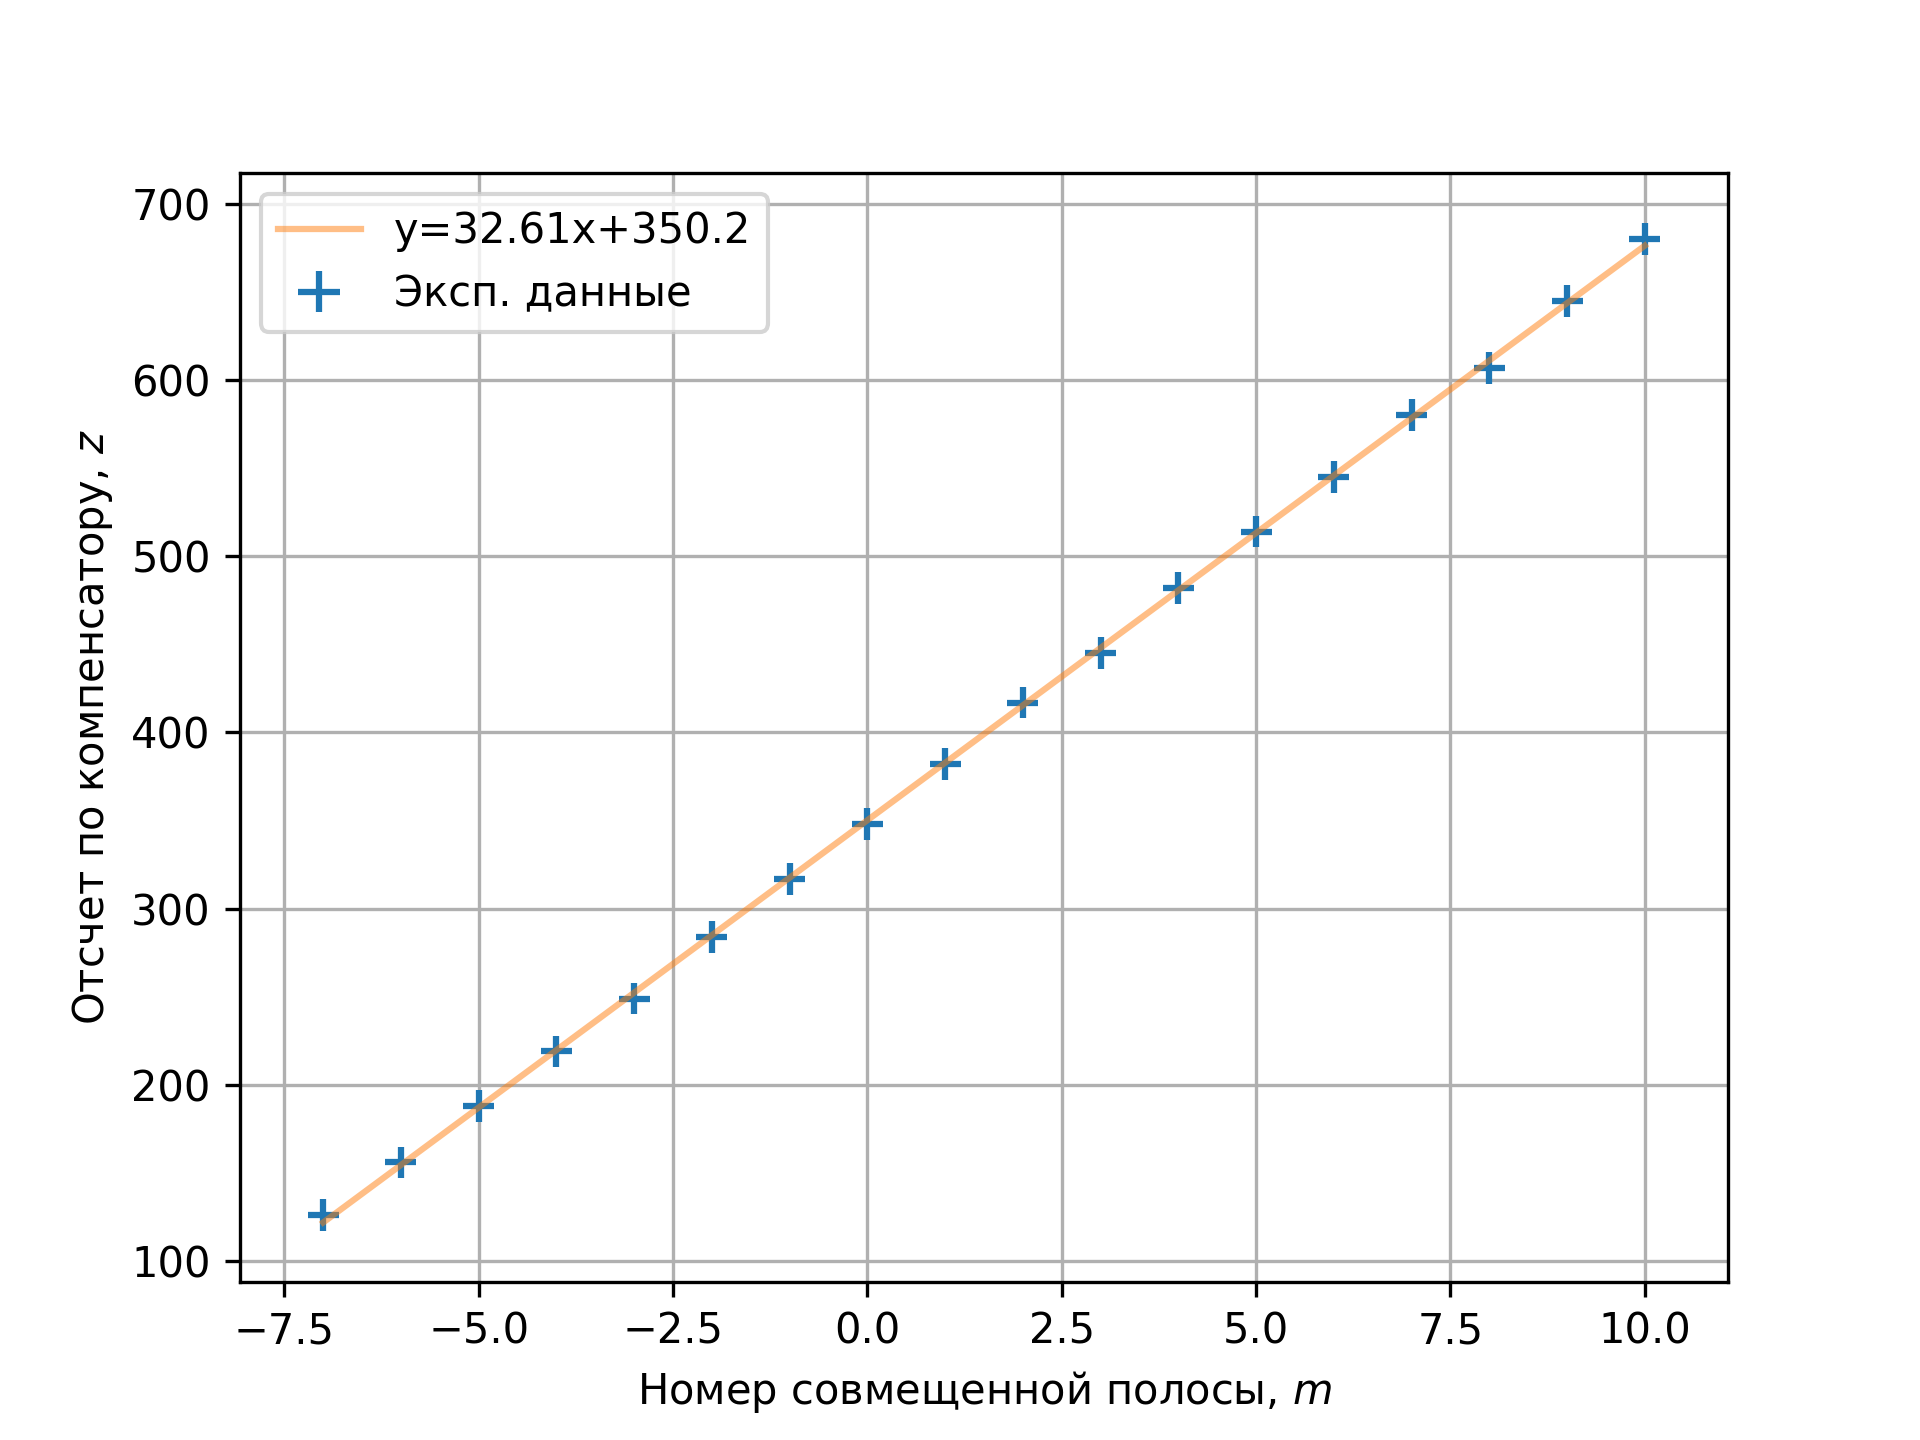
\includegraphics[width=\linewidth]{pic/3-5}
        \label{fig:fig2}
    \end{minipage}
    \hfill
    \begin{minipage}[t]{0.5\linewidth}
        \centering
        \caption{Рис. 3: Зависимость $\delta n$ от $\Delta P$}
        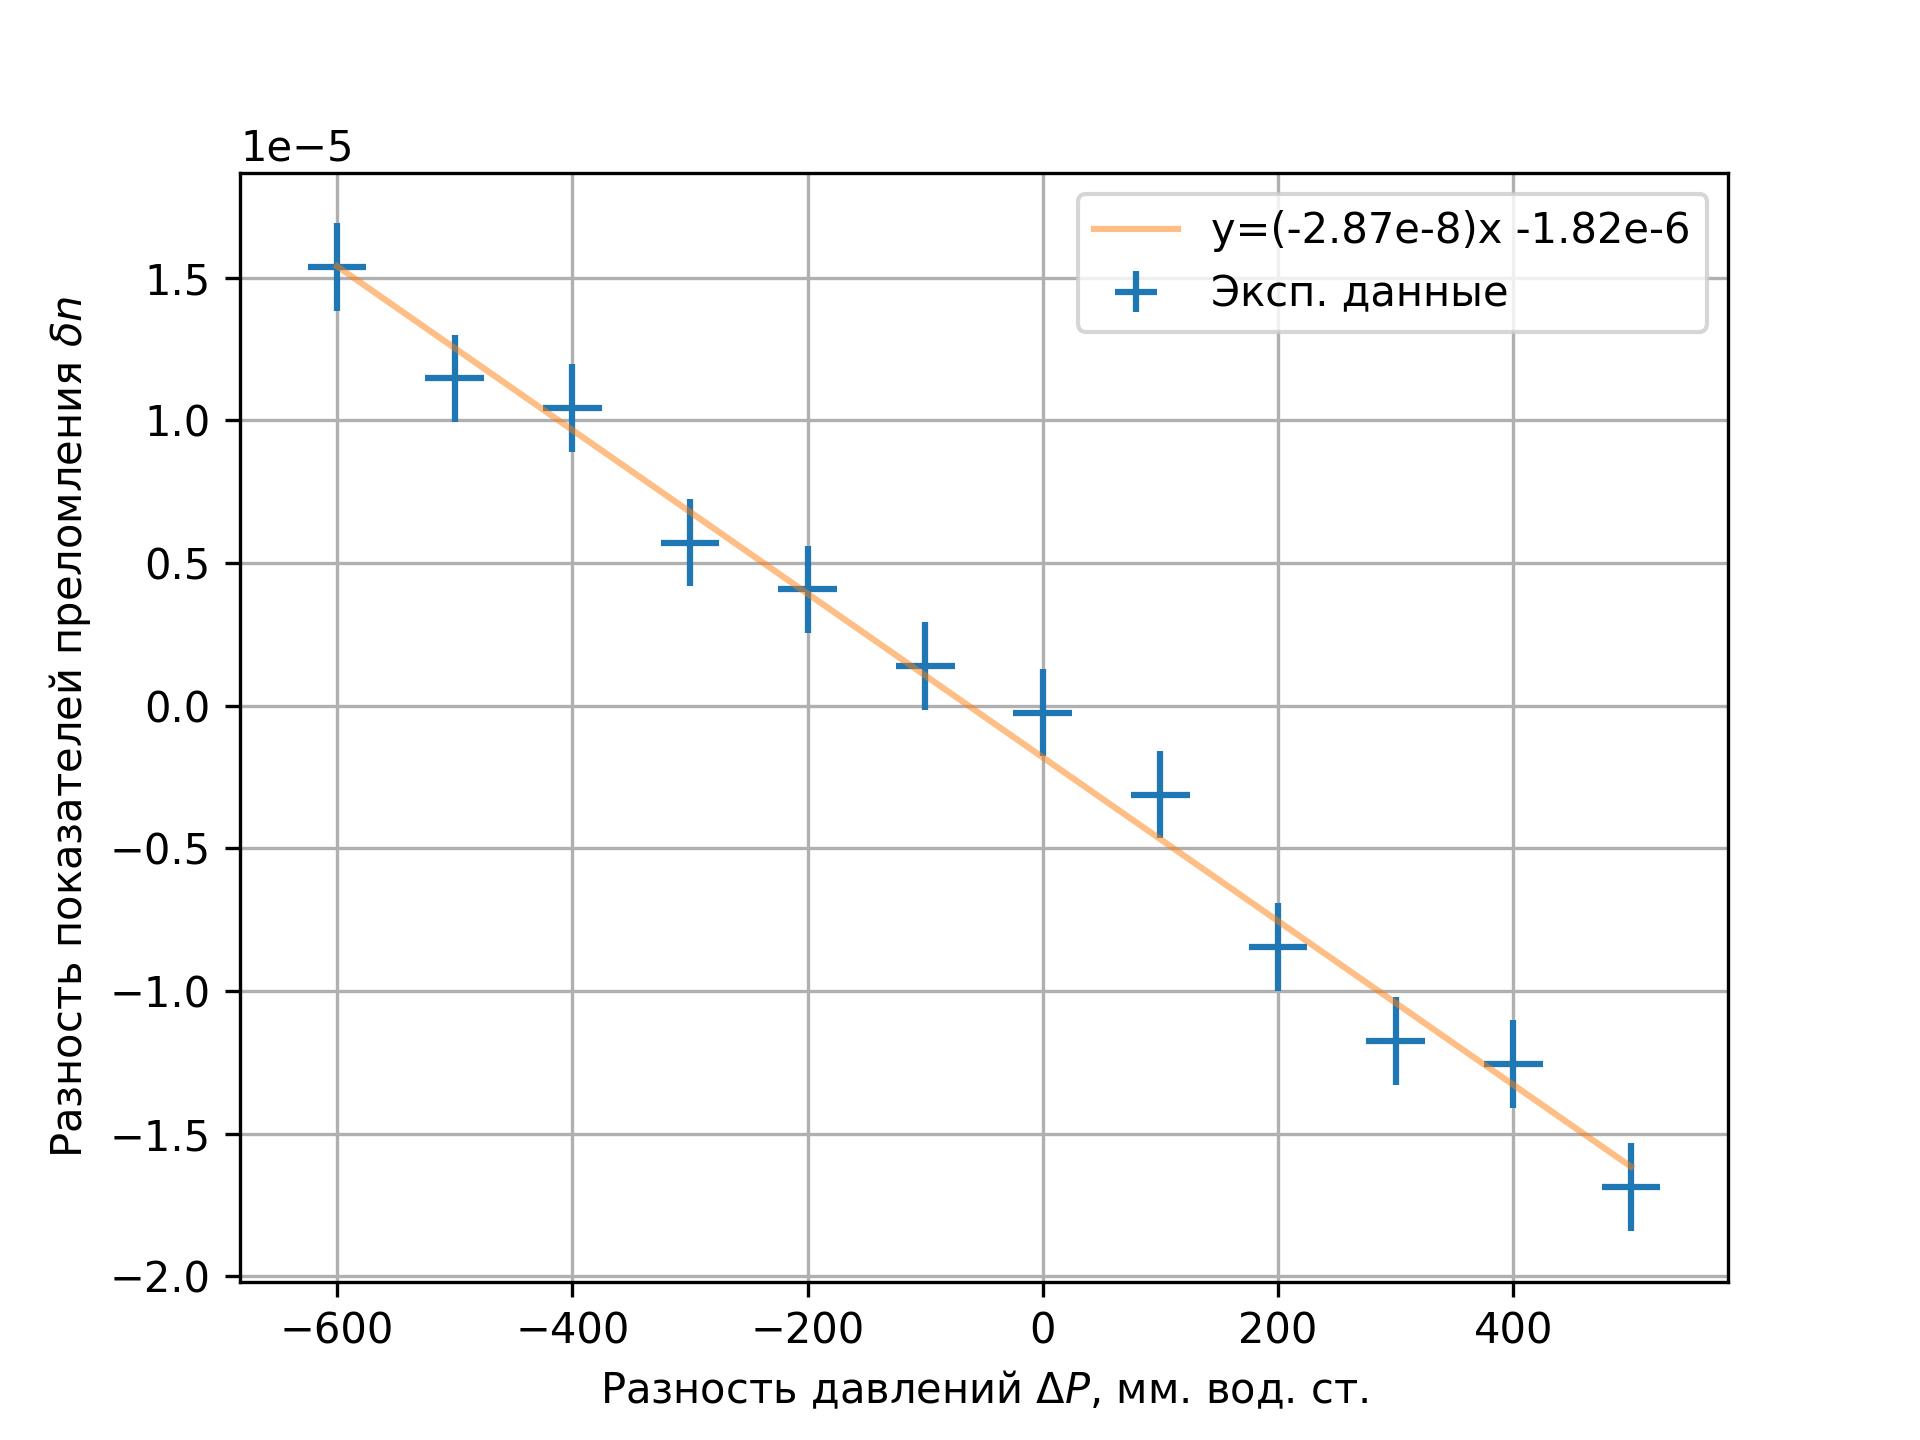
\includegraphics[width=\linewidth]{pic/6-7}
        \label{fig:fig3}
    \end{minipage}
    \vfill
    \begin{minipage}[t]{0.2\linewidth}
        \centering
        \caption{Таблица 1: Калибровка компенсатора}\\
        \label{tab:tab1}
        \begin{tabular}{|l|r|r|}
            \hline
            & m  & z   \\
            \hline
            0  & 0  & 348 \\
            1  & 1  & 382 \\
            2  & 2  & 417 \\
            3  & 3  & 445 \\
            4  & 4  & 482 \\
            5  & 5  & 514 \\
            6  & 6  & 545 \\
            7  & 7  & 580 \\
            8  & 8  & 607 \\
            9  & 9  & 645 \\
            10 & 10 & 680 \\
            11 & -1 & 317 \\
            12 & -2 & 284 \\
            13 & -3 & 249 \\
            14 & -4 & 219 \\
            15 & -5 & 188 \\
            16 & -6 & 156 \\
            17 & -7 & 126 \\
            \hline
        \end{tabular}
    \end{minipage}
    \hfill
    \begin{minipage}[t]{0.4\linewidth}
        \centering
        \label{tab:tab2}
        \caption{Таблица 2: Зависимость $\delta n$ от $\Delta P$}
        \begin{tabular}{|l|r|r|r|r|}
            \hline
            & $\Delta P$ & $z$ & $m$   & $\delta n,\ \cdot 10^{-5}$ \\
            \hline
            0  & 0          & 349 & -0.03 & -0.02                      \\
            1  & 100        & 335 & -0.46 & -0.31                      \\
            2  & 200        & 309 & -1.26 & -0.84                      \\
            3  & 300        & 293 & -1.75 & -1.17                      \\
            4  & 400        & 289 & -1.87 & -1.25                      \\
            5  & 500        & 268 & -2.52 & -1.68                      \\
            6  & -100       & 357 & 0.20  & 0.13                       \\
            7  & -200       & 370 & 0.60  & 0.40                       \\
            8  & -300       & 378 & 0.85  & 0.57                       \\
            9  & -400       & 401 & 1.55  & 1.04                       \\
            10 & -500       & 406 & 1.71  & 1.14                       \\
            11 & -600       & 425 & 2.29  & 1.53                       \\
            \hline
        \end{tabular}
    \end{minipage}
    \hfill
    \begin{minipage}[t]{0.3\linewidth}
        \centering
        \caption{Таблица 3: Зависимость равновесного положения компенсатора от времени}
        \label{tab:tab3}
        \begin{tabular}{|l|r|r|}
            \hline
            & $T$, с & z   \\
            \hline
            0 & 0      & 294 \\
            1 & 60     & 315 \\
            2 & 120    & 345 \\
            3 & 180    & 345 \\
            \hline
        \end{tabular}

    \end{minipage}
\end{document}